\documentclass[fleqn,12pt]{wlscirep}


\usepackage[utf8]{inputenc}
\usepackage[T1]{fontenc}
\usepackage{setspace}
\usepackage{newtxmath,newtxtext}

\usepackage{comment}
\usepackage{subfig}
\usepackage{wrapfig}
\usepackage[square,sort,comma,numbers]{natbib}
\usepackage{pdfpages}





\onehalfspacing
\graphicspath{ {images/} }
\begin{comment}
Things to do: 
add figures to illustrate LSM

write intro
add literature review criticisms

add readout neuron training algo comparison with figures
finish last para
add conclusion
^^ finish technical progress section

Add gantt chart and gantt chart references and review project progress section

Is the self review ok to be in the first person ??
review self review

label figures
add figure references using ref command
fix all citations
\end{comment}


\title{Interim Report: Biologically inspired Spiking Neural Networks for Signal Processing and
Classification}

\author[1]{Caleb Parikh}

\affil{University of Sheffield,Automatic Control Systems Engineering}

%\keywords{Keyword1, Keyword2, Keyword3}


\newpage
\begin{abstract} 

\end{abstract}
\newpage

\begin{document}


\flushbottom

\maketitle

\thispagestyle{empty}

\newpage
\section*{Background to Project}
Computational neuroscience uses mathematics to gain a better understanding of the underlying principles that govern the cognitive abilities of the brain \cite{noauthor_computational_nodate} and is focused on describing biologically plausible neurons. Although upon initial inspection computational neuroscience can seem overtly abstract \cite{singer_neuronal_1999} \cite{cleland_computation_2005}
the insight that computational neuroscience provides, through mathematically rigorous description, of the brains physiology, has shown promise in the diagnosis and treatment of neurodegenerative diseases \cite{huys_are_2011} and is becoming increasingly used in psychiatry \cite{huys_computational_2016} (although it is worth noting the limitations of these models, as is often seen outside of typically non-mathematically settings \cite{huys_are_2011}). 

In addition to this neuroscience is beginning to become increasingly useful in the advancement of core machine learning research \cite{marblestone_towards_2016} \cite{hassabis_neuroscience-inspired_2017}, although, this is removed from focus of the field and should be treated as only a potential byproduct of advancement in the field \cite{eliasmith_use_2014}. In machine learning artificial neural networks use connected perceptrons as a framework for algorithms to process data through \cite{noauthor_build_nodate}. There are a variety of transfer functions that are used in these networks but sigmoidal functions are the most common, possibly due to their easily calculable derivative which is central to training using backpropagation \cite{duch_survey_1999}. Neural networks composed of spiking neurons, have become increasingly popular, due to the biological plausibility of transfer functions in spiking neurons \cite{long_review_2010}. Sufficiently complex networks of spiking neural networks are likely to be capable of accurately modelling the  cognitive function of the human brain, although current computer power is considered insufficient  for this task \cite{noauthor_brain_nodate}. As is common in life sciences, a good starting point is a model organism such as Mus Musculus (house mouse) or in our case Drosophila Melanogaster (fruit fly).

\section*{Aims and Objectives}
This projects aims to develop and evaluate biologically inspired spiking neural network models that implement signal processing and classification tasks performed by the sensory processing areas of the fruit fly brain.

Objectives for this project are broadly split into two categories; basic and advanced objectives. They were  established in a previous component of the project but particular attention has been drawn to any modifications.

\subsection*{Basic Objectives}
\begin{itemize}
  \item Review the literature surrounding models of spiking neurons, particularly liquid state machines, and the fruit fly early visual system. The focus of the literature review has moved away from comparisons to artificial neural networks so as to narrow the focus of the project.
  \item Evaluate the state-of-the-art  spiking neural network (SNN) training algorithms.
  \item Develop and validate a biologically inspired SNN model of the early visual system in Drosophila
\end{itemize}

\subsection*{Advanced Objectives}
\begin{itemize}
    \item Develop and validate an SNN model of other sensory processing systems
    \item Investigate the influence of network connectivity on classification performance
\end{itemize}

\section*{Literature review}

\subsection*{Introduction}
Drosophila melanogaster (fruit fly) are often used as a model organism for a variety of research including animal development, genetic diseases and neurobiology. They are often used to model brain diseases in humans, and invertebrate models such as these do offer some significant advantages over rodent models. It is likely that accurate models in the future will provide great insight into treatments for neurodegenerative diseases including Alzheimer's and Parkinson's disease, as well as providing insight into new genetic pathways producing molecular based therapy approaches \cite{jeibmann_drosophila_2009}. This project is focused on modelling the visual processing system in fruit flies. This literature review will aim to give an overview of the structure and function of the early visual system in drosophila melanogaster, as well as the current progress in biologically plausible neural networks with particular focus drawn to the novel computing framework, the liquid state machine.


\subsection*{The early visual system of the fruit fly}
In many arthropods (such as flies) the compound eyes are composed of clusters of photoreceptors called ommatidium. It is believed that each ommatidium provides one element of the image. The portion of photoreceptors on the central axis of the ommatidium form a transparent tube called the rhabdom, which in turn is separated into multiple independent rhabdomeres consisting of thousands of microvilli \cite{song_stochastic_2012}. 
%figure showing drosophila eye structure 
\begin{wrapfigure}{l}{0.6\textwidth}
    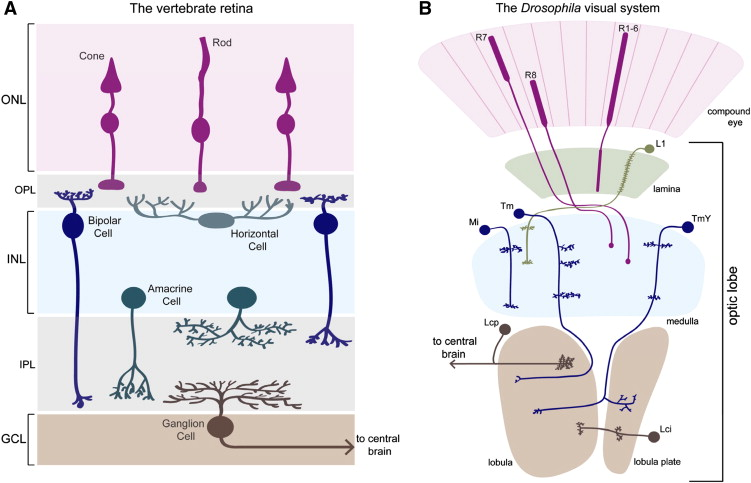
\includegraphics[width=8cm]{flyVisSys.jpg}
    \centering
    \caption{Structure of the Drosophila Early Visual System\cite{erclik_eye_2009}}
    \label{fig:structure}
\end{wrapfigure}
Each villi respond individually using a phototransduction cascade (chain of biochemical events along a signalling pathway) which has stochastic characteristics. This cascade is thought to be understood \cite{kiselev_molecular_2000} but significantly less is known about how information on light changes is encoded in the resulting electrical signal.
The R1 - R6 photoreceptors project to the lamina whilst the R7 and R8 photoreceptors reach deeper into the medulla \cite{zhu_drosophila_2013}. 


The lamina and medulla along with the lobula and lobula plate are the four neuropiles that make up the optic lobe \cite{morante_color_2008}. The medulla is thought to be responsible for colour vision \cite{morante_color_2008} whereas the lamina is thought to handle tasks more critical for useful sight, primarily edge detection.

Previous work has been done to generate biophysically realistic photoreceptor models. These are capable of simulating the encoding of visual information accurately and shows how adaptive sampling of microvilli captures natural contrast changes \cite{song_stochastic_2012}. It was postulated that sensory pathways are tuned to selectively enhance certain characteristics that are critical to survival, but it is very difficult to fully characterise these signals.  One problem with this postulate is that although it is based on good reason, it is very difficult to design experiments to verify this hypothesis, without fully characterising these signals, which of course is the reason for the postulate. It has, however, been shown that R1-R6 photoreceptors encode points of maximum and minimum local phase congruency that are critical for edge detection \cite{friederich_fly_2016} and thus have particular biological relevance and support the postulate.

This project will build on this work to suggest biologically plausible models for the type of characterisation carried out in the parts of the optic lobe (focusing on the lamina and medulla), primarily based around the liquid state machine.

\subsection*{Visual tasks}
In order to validate the model, appropriate input and output data will need to be collected. As discussed above there are a number of statistically relevant features that should provide a minimum set of requirement for the function of the model, derived from postulate that sensory neurons selectively enhance some subset of features that are deemed useful to survival by evolution \cite{friederich_fly_2016}\cite{simoncelli_natural_2001}. It is therefore sensible that data that reflects this is used. One weakness in this approach is in identifying sensible traits, however, the majority of the literature is in agreement so it is unlikely to be of concern. The first iteration of the model will be framed as a classification problem of videos containing bands moving in different directions. The important feature of this data is that it is temporal in nature, and the moving edges of the gratings are the key indicator for which to classify by. Similar forms of dynamic pattern classification using echo state networks has shown good results in previous papers \cite{tanaka_recent_2018}.

\subsection*{Overview of Liquid State Machines}
\begin{wrapfigure}{l}{0.5\textwidth}
    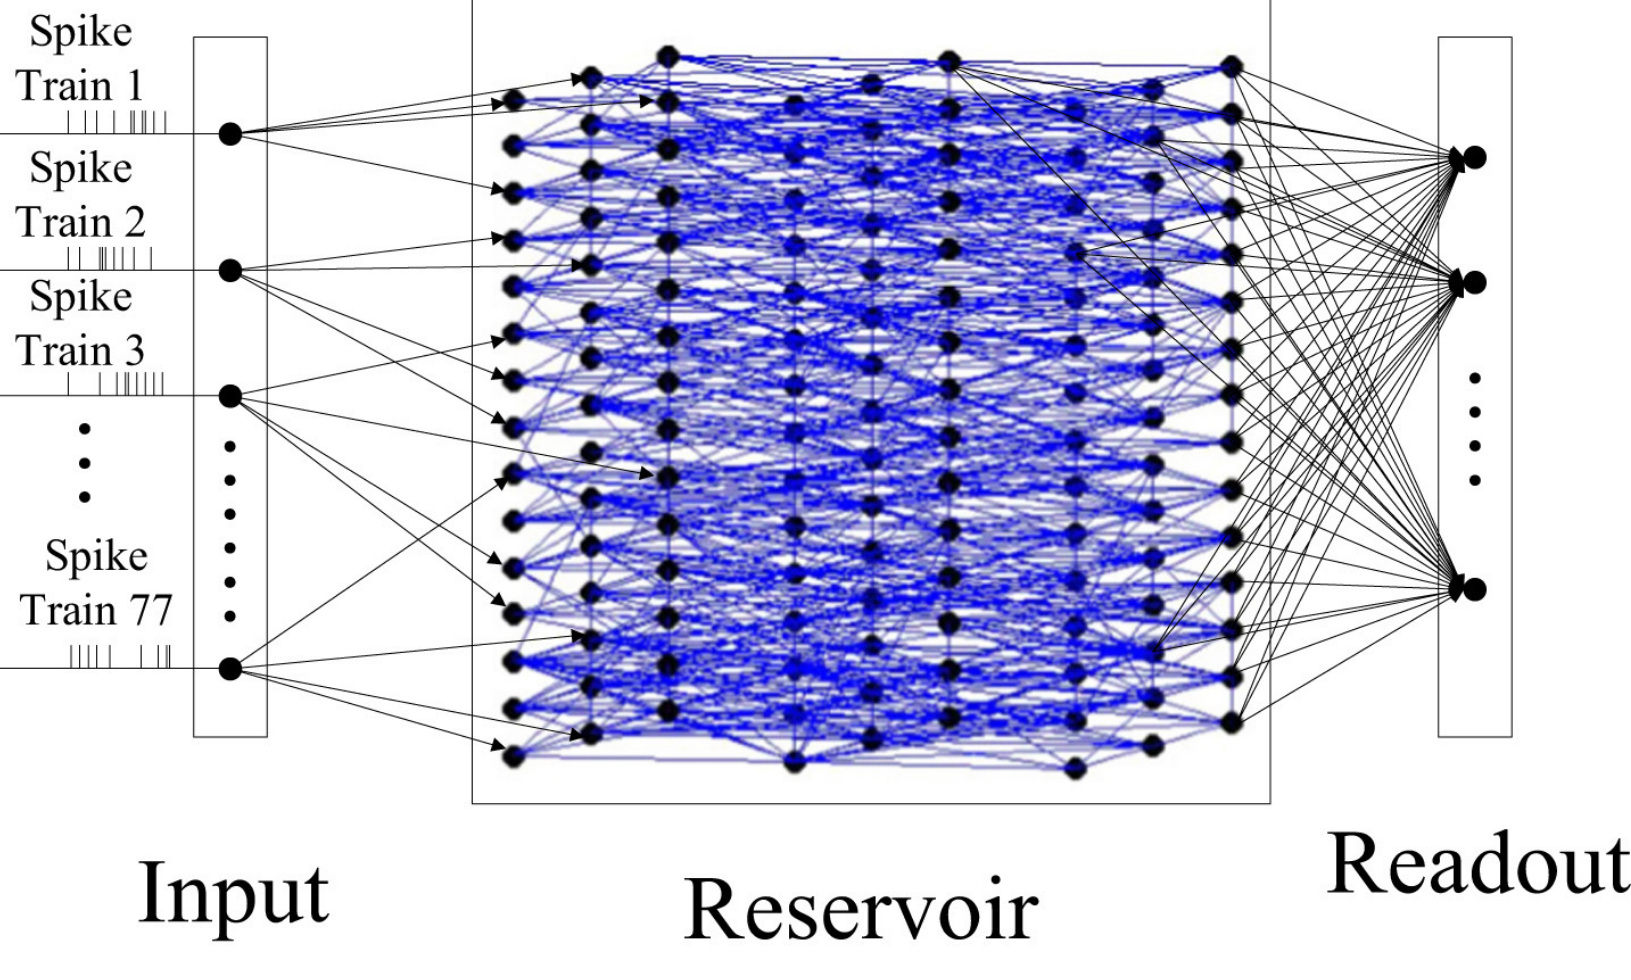
\includegraphics[width=8cm]{lsm.png}
    \centering
    \caption{Structure of the Liquid State Machine System\cite{jin_performance_2017}}
    \label{fig:LSM}
\end{wrapfigure}
Liquid state machines are recurrent neural networks (RNN's) that provide a more biologically plausible model for the the brain compared to conventional artificial neural networks \cite{yamazaki_cerebellum_2007}. Liquid state machines differ to artificial neural network models in that they are composed of spiking neurons, the dynamics of which are derived from the behaviour of biological neurons. Spiking neurons can be loosely defined as a summation which, when it reaches a threshold, fires and produces a raised potential at the output. 

They are sometimes referred to as the ‘third generation of neuron’ \cite{maass_networks_1997} and have been shown, with regards to the number of neurons needed, to be more computationally powerful than models base on McCulloch-Pitts neurons. One of the limitations of these netowrks , is that they  are very computationally expensive  are to train, which is sometimes glossed over in papers investigating SNN's. They, along with echo-state networks, introduce a new framework for computation called reservoir computing \cite{jaeger_echo_nodate}
\cite{maass_real-time_2002}. 

Fundamentally the input signal is fed into a randomly connected RNN which is then fed into a read out layer, but only the read out layer is trained. The principle is analogous to a stone being dropped into a physical liquid reservoir, characteristics of the stone can be inferred from the shape of the ripples, as the reservoir provides a mapping from the input into a higher dimension \cite{schrauwen_overview_nodate}.

\subsection*{Training algorithms for liquid state machines}
Backpropagation is possibly the most common method for training conventional feedforward networks. At the core of backpropagation in computing the error gradients so that weights in the network can be adjusted accordingly. There are many adaptations to this gradient descent approach to avoid local error minima as well as speed up the training of the network 
\cite{jaeger_tutorial_nodate}
. As recurrent neural networks contain feedback loops, feedforward backpropagation cannot be directly applied to the network, one approach is to unfold this network in time. This expands the network the stacking identical copies of the recurrent network to give a feedforward network. The resulting feedforward network can then be trained using back propagation, this approach is known as backpropagation through time
\cite{jaeger_tutorial_nodate}
. Unfortunately it is very computationally intense. Other approaches exist including real-time recurrent learning and higher order gradient descent techniques that make use of the curvature of the function to be optimised.

Reservoir computing offers an alternative to these methods. Assuming that the reservoir is damped (so that the behaviour of the system in stable), the training is performed by first writing the desired outputs on the read out neurons (teacher forcing) and then computing weights for the readout neurons such that the desired output is approximated by a linear combination of the internal activation time series 
\cite{jaeger_tutorial_nodate}.

Although normally only the readout neurons in an LSM are trained, there have been some attempts to train the reservoir in order to create some structure in the liquid, allowing for a more effective mapping from temporal data to spatial data using Hebbian learning, some literature notes a significant improvement in separation (which refers to the robustness of the model to respond differently to different classes of input) with only a small amount of training (1-3 iterations) but further training iterations produced negligible returns 
\cite{norton_preparing_nodate}, it is worth noting that the literature supporting this is limited to a handful of papers, and because of this it is worth being cautious of it's reproducability on generic tasks (tasks outside the realms of the paper)
.

Generally the readout neurons are trained via simple linear regression by solving a system of linear equation, but weighted regression and evolutionary methods have also been employed but at a much higher computational cost \cite{lukosevicius_reservoir_2009}.

It is worth noting that the above methods seem unrealistic from a neuroscience perspective but there has been some progress in algorithmic learning rules that are more biologically plausible, notably target prop and EM updating \cite{bengio_towards_2015}. Reinforcement learning also presents an interesting paradigm for learning that has been shown some favour by neuroscientists as biologically plausible and has been demonstrated as a viable way of training networks of spiking neurons [missing reference for biologically plausible reinforcement learning][missing reference for spike time dependent plasticity reinforcement learning paper].

\subsection*{Conclusion}
The findings of this literature review indicate that liquid state machines would be a suitable model for components of the early visual system in drosophila melanogaster. The lamina is of particular interest to model, as it is responsible for type of characterisation of signals most critical to sight. Suitable visual tasks will need to be designed in order to validate the model and visual tasks should reflect the important features of sight from an evolutionary perspective (such as edge detection).



\section*{Work Progress to Date}
In order to achieve the objectives previously presented, networks of spiking neurons need to be simulated. In order to do this an LSM MATLAB toolkit from Tu Graz was used. Installing the toolkit proved more difficult than expected, as it is no longer maintained. Some of the source code needed modifying and many of the dependencies written in c++ needed compiling for 64 bit operating systems (all modifications will be made available via GitHub) but, eventually the toolkit was installed successfully

The first step was to simulate a single spiking neuron (leaky integrate and fire). LIF neurons 'fire' when their membrane reaches a certain potential, their dynamics can be described in the following equations. 
$$I(t) - \frac{V_m(t)}{R_m} = C_m \frac{dV_m(t)}{dt}$$ 
Where $I(t)$ is the current wrt. time, $V_m(t)$ is the voltage of the membrane, $C_m$ is the capacitance of the membrane and $R_m$ is the membrane resistance.

The LIF neuron was driven by a Poisson spike train transmitted through a synapse. This was done by creating all three parts in the configuration in figure (a).

\begin{figure}[ht]
    \centering
    \subfloat[Model Setup for Testing of Single Neuron]{{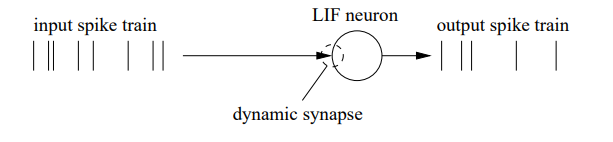
\includegraphics[width=8cm]{singleNeuronSetup.png} }}
    \qquad
    \subfloat[Analysis of Single Neuron Test]{{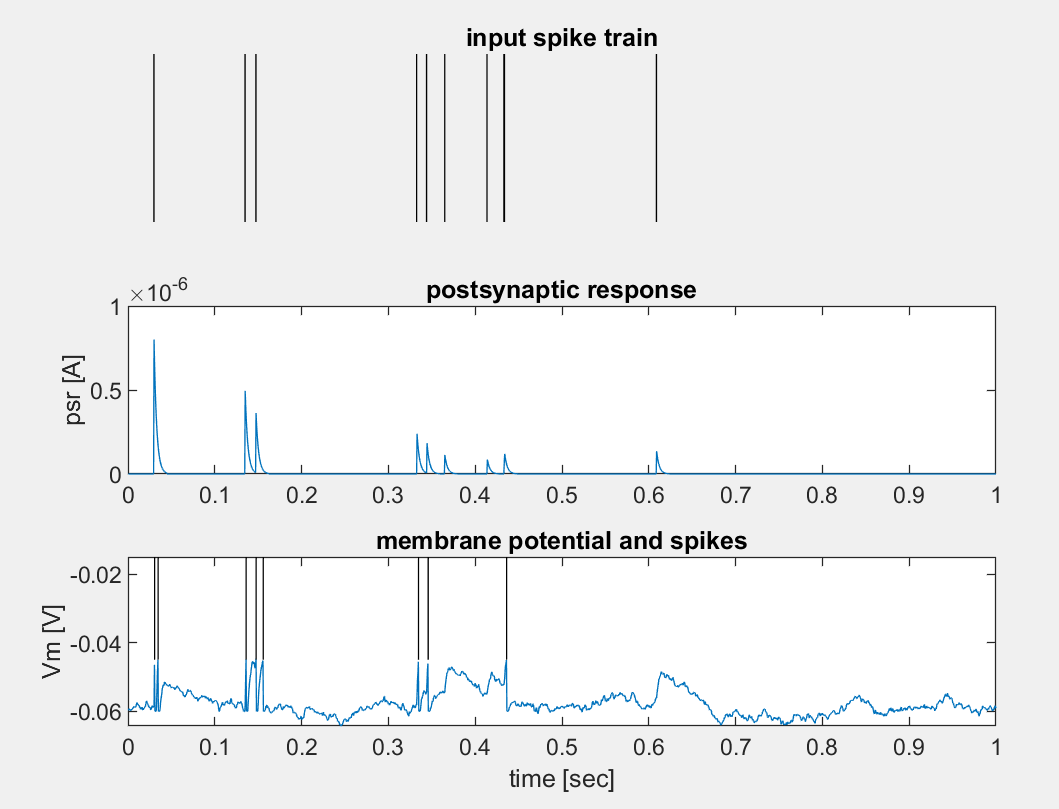
\includegraphics[width=6cm]{spikeTrainNeuron.png}} }
    \label{fig:SingleNeuronFigures}
\end{figure}

Figure (b) was generated showing the output of the postsynaptic neuron and the output membrane potential notice that the output spikes, whenever a critical potential is hit.

The next step was to set up a liquid state machine on a relatively simple task using the LSM toolbox from TuGraz \cite{noauthor_neural_nodate}. The task for our base case was for readout neuron (representing a presynaptic neuron) to differentiate between two, input spike train signals. Two templates of Poisson spike trains were generated at 20 Hz with a length of 0.5s, these parameters are reasonably arbitrary, but they are a good representation of the type of signal that will be processed by the model later in the project, and was not hugely computationally intense. Some noise was added to each each spike, the amount of noise added was taken from a Gaussian distribution with zero mean score and a standard deviation of 4ms. This is to increase the similarity of our spike train to typical spike trains generated in fly photoreceptors \cite{song_stochastic_2012} although this technique is commonly used to prevent overfitting in machine learning tasks. The model used a single readout neuron, modelled as a threshold gate, with the task of outputting a 1 or 0 corresponding to the randomly selected input template. The readout neuron was trained offline (where the data set is static and data is fed into the LSM in batches rather than continuously as data is made available). This meant that first the response of the neural circuit was measured using appropriate training inputs from the aforementioned distribution. These were then passed through a low pass filter, sampled and converted into states. This has the effect of smoothing the signal, and, is similar to the preprocessing that occurs when the signal is passed through a synapse, and high frequency noise components are lost. A supervised learning algorithm is then applied to the set of training examples so that the readout function mimics the target function as closely as possible.

 A variety of supervised learning algorithms were applied including linear classification, p-delta \cite{auer_p-delta_nodate}
 , linear regression, and backpropagation in order to compare their performances on the sample data set. This important computationally but it is worth noting that the biological plausibility of these algorithms in generally criticised by the neuroscience community, more plausible biological learning rules , particularly reinforcement learning techniques, do exist [4] and their application to this project is likely to be investigated in future work. These training algorithms were compared, a brief summary of results can be found below with respect error (by mse score) and a preliminary discussion of these results.

\begin{figure}[ht]
    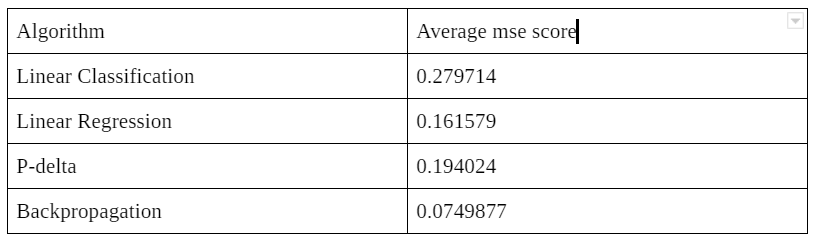
\includegraphics[width=8cm]{algoComp.png}
    \centering
    \caption{Preliminary Results of LSM training for different Algorithms}
    \label{fig:trainingAlgoResults}
\end{figure}

As shown in the figure, backpropagation gave the best performance, however it is worth noting that the P-delta method and backpropagation both took far longer to run that the linear regression and classification algorithms. 

\begin{figure}[ht]
    \centering
    \subfloat[Response of readout neuron for various training algorithms]{{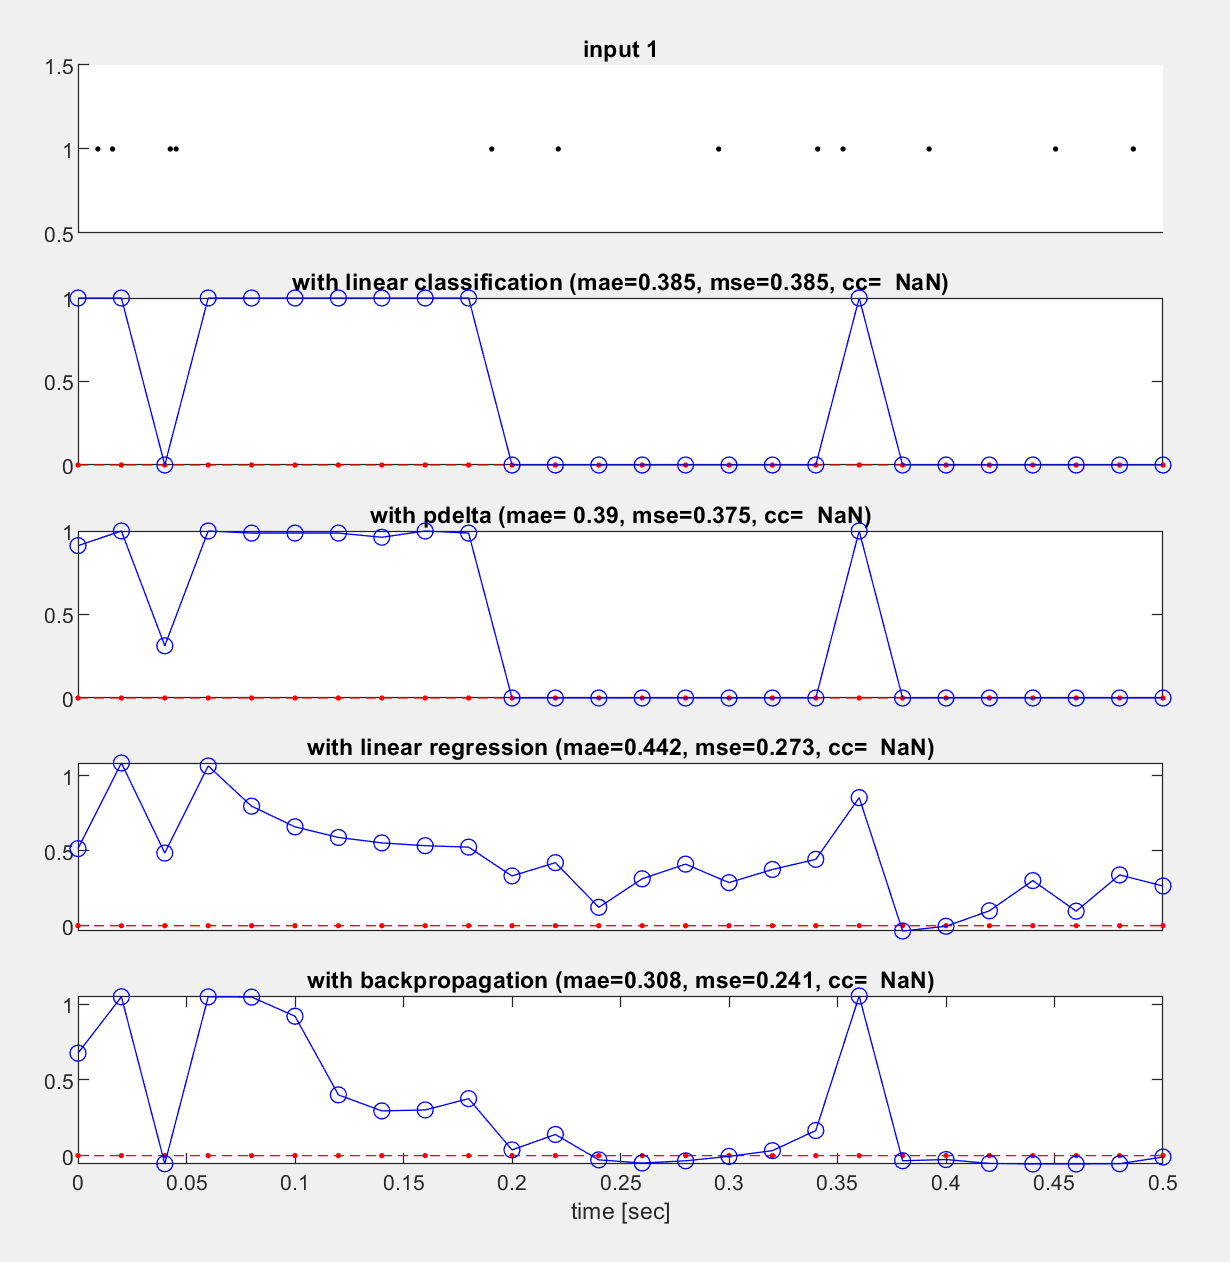
\includegraphics[width=6cm]{algoResp.png} }}
    \qquad
    \subfloat[Accuracy of backpropagation trained readout neuron for various iterations on validation set]{{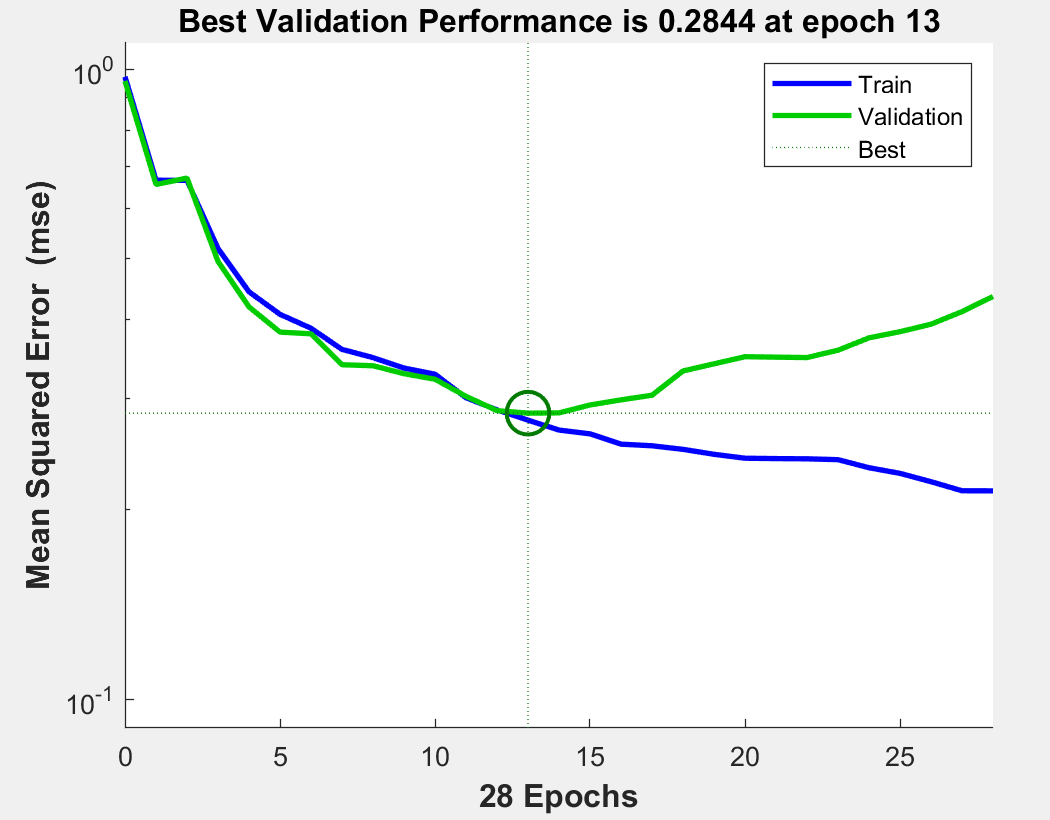
\includegraphics[width=8cm]{valPerfBP.png} }}
    \label{fig:LSMAnalysis}
\end{figure}

Upon further investigation of the backpropagation algorithm, it looks like there is some over-fitting, if run for too many iterations. In this case we can use the validation set to chose the iteration with the best performance.

The base case task was then expanded to a more sophisticated example, more directly linked to the previously identified requirements for visual tasks in this context. Moving bands moving in one of 12 directions are to be classified by the neural network. There a few key challenges presented by the new task. Firstly each moving band pattern encodes temporal information which is key to distinguishing between different directions of motions. LSM’s are suited to this kind of information processing as spike trains are inherently temporal in nature so minimal modifications need to be made to our network. More significantly, the task is no longer a binary classification task requires distinction between 12 different classes. The architecture of the network was modified by adding 11 read out neurons to allow the network to differentiate between each class. Currently the model has been implemented but no validation has been done using the moving bands data.

In summary progress has been made in successfully rewriting and testing the source code for the LSM toolbox, constructing simple circuits with spiking neurons and larger liquid state machines and applying a variety of training algorithms to the read out neurons in a classification task. Some progress has been made to classify temporal data, but this is waiting for validation.

\section*{Project Management}
Referring back to the aims and objectives of the project, there has been a significant amount of progress made on the basic objectives. The majority of the literature review has been completed for both the spiking neuron models and fruit fly visual system. Implementing the preliminary iterations of the model means that the SNN training algorithms can now be evaluated and some evaluation of training algorithms with respect to the read out neurons has been achieved. The full model of the early visual system is still in progress and as of yet has not been validated. There has however been concrete progress made in this area, most notably, a liquid state machine was successfully simulated and recorded with one read out neuron. The liquid was excited with a spike train and the readout neurons were trained to distinguish between two types of signal. In order to achieve the final basic objective, the model must be extended to multiple read out neurons, and the moving bands data must be used to excite the liquid, some progress has been on the latter point, as this data has been converted to spike trains which the network can interpret. After this is done there will need to be some validation using the same methods as used in the single readout neuron model. In order to progress to the advanced objectives the literature review must be extended to olfactory processing in fruit flies. It is likely that structure of the network will be similar but literature will be required to verify this and new data will need to be sourced in order to validate the model. The second semester gantt chart has been updated accordingly to add more time for this task, and ensure that software issues are run in to, then there is some leeway that can be used.

In order to tackle the final advanced objective various network will need to be generated at various connectivity's. In the initial model the probability of two neurons being connected decreases exponentially with distance according to the formula, $p = C \cdot exp\left[\frac{D(a,b)}{\lambda}^2\right]$
where $\lambda$ is a connection parameter, and $D(a,b)$ is the Euclidean distance (straight line distance) between neurons a and b.
There are however other network topologies such as small world networks \cite{watts_collective_1998} and axon models \cite{yamamoto_wiring_2002} where neuron connections are defined by different parameters. In order to compare various topologies, networks will be created and results of a common classification task will be compared. The second semester gantt chart has been updated accordingly. The task associated with this objective has been split into smaller objectives so as to provide more detailed guidance of time allocation.


\section*{Self-review}
Although I am satisfied with the progress that I have made with respect to the aims and objectives, one issue I faced concerned the amount of uncertainty surrounding completion of sub tasks. For example it took me far longer than expected to install the MATLAB toolbox due to having to re-factor some of the source code and recompile various c++ files. However, there were some parts, particularly the initial classification tasks, that were completed much more quickly than expected. I am used to working in an agile manner in situations like these where there is some degree of uncertainty, allowing me iterate at a high level and be reasonably fluid with decisions within a project. One way in which I plan on rectifying this issue in the future is by better breaking down problems into steps I can tackle in an agile manner, so that robust progress can continuously be made.

Another area in which I feel that I can improve on is optimising meetings. At the start of the process meetings with my supervisor, although in the moment felt productive, sometimes lead to intangible progress. Results were sometimes difficult to take action on and progress was therefore hard to measure. One way that we have improved this is by dedicating time at the end of meetings to designing concrete steps that can be taken over the next few weeks similar to sprints in agile. So far throughout the process I have been using the ‘getting things done’ framework through the app ‘Trello’, this has helped me break down tasks into small components, and lets me track my own progress much more easily. In the future, it may be beneficial to share the Trello board with my supervisor of do weekly write ups, based on these boards to increase the frequency at which I receive feedback in a time efficient manner. One suggestion my supervisor had for me was to write a brief document preceding each meeting with a progress update and an outline of the questions I would like answers to in the meeting, so as to now waste time catching up on progress at the start of each meeting.

\bibliographystyle{plainnat}
\bibliography{interimReport2}

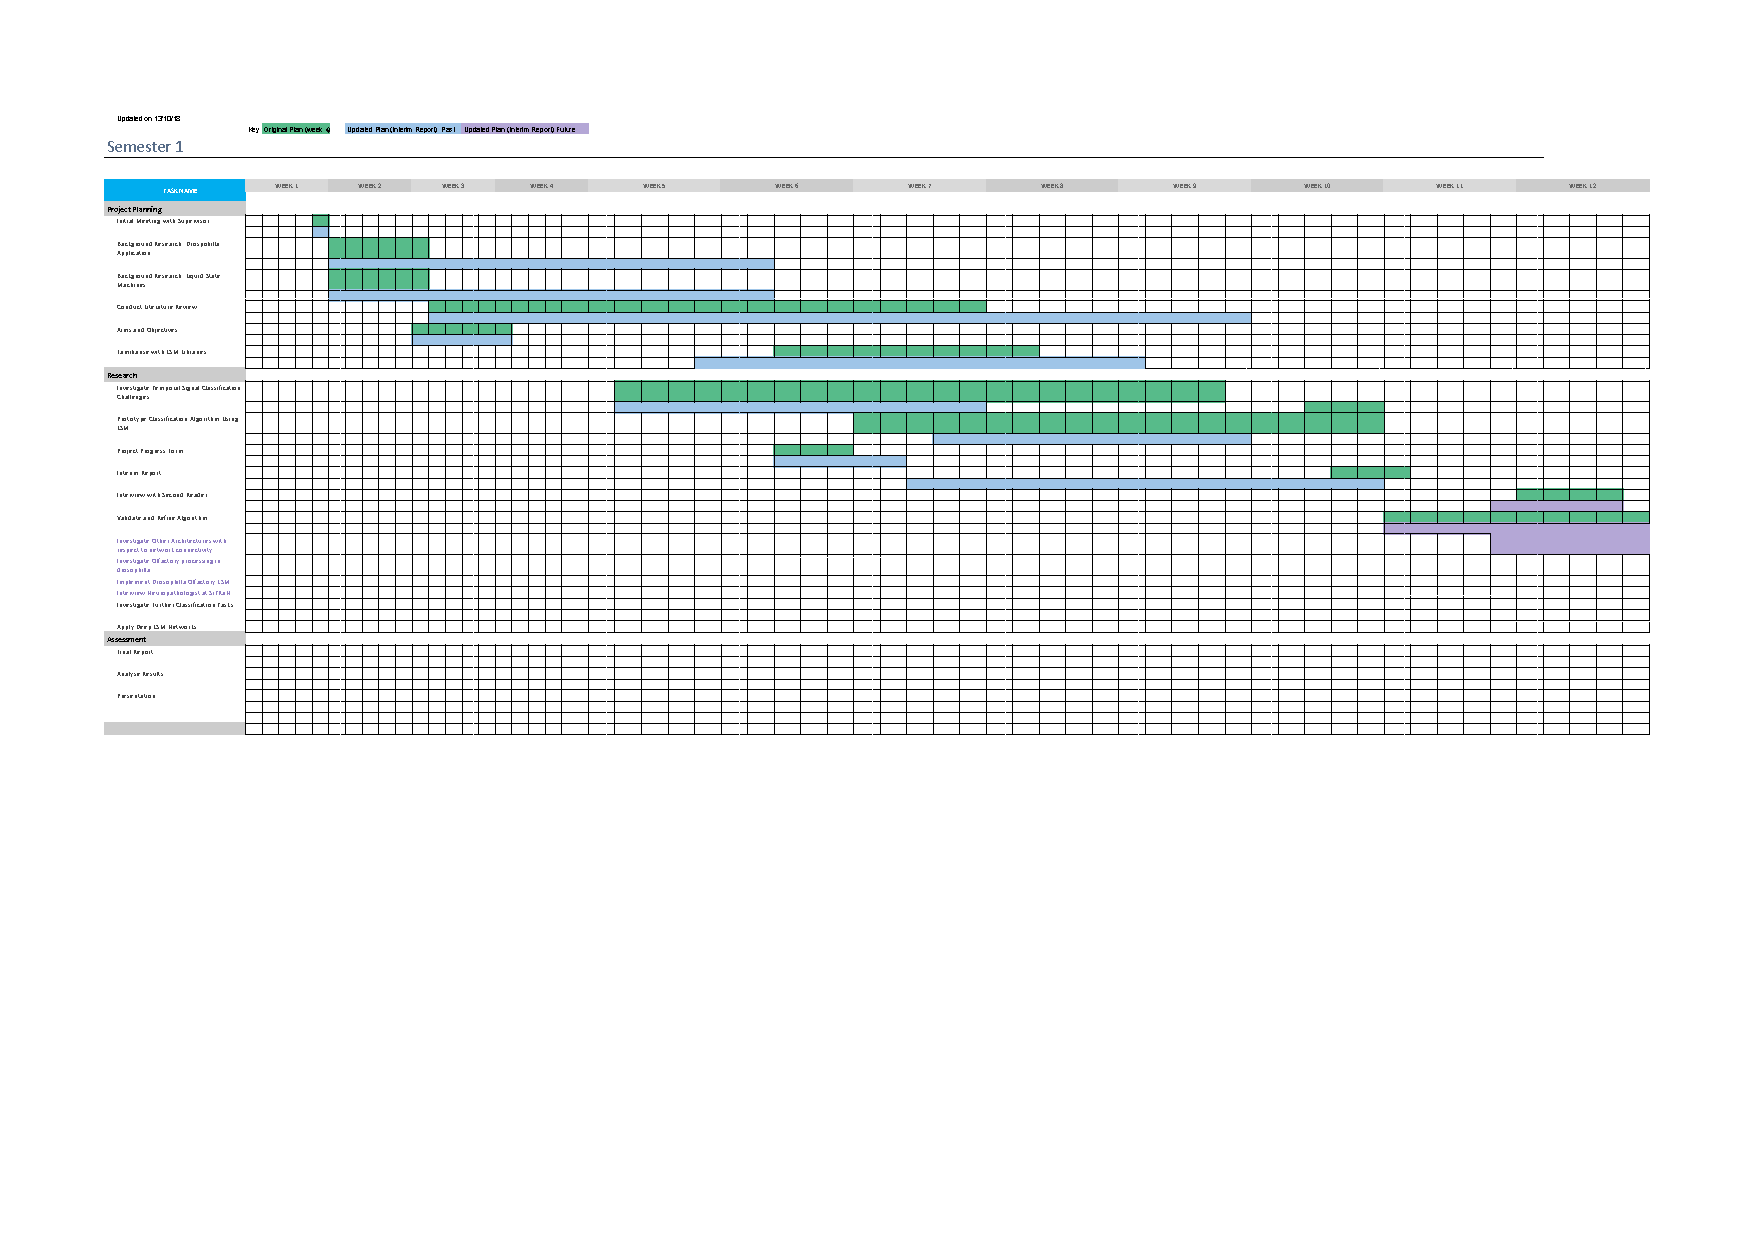
\includepdf[pages=-,angle=90]{chart1.pdf}
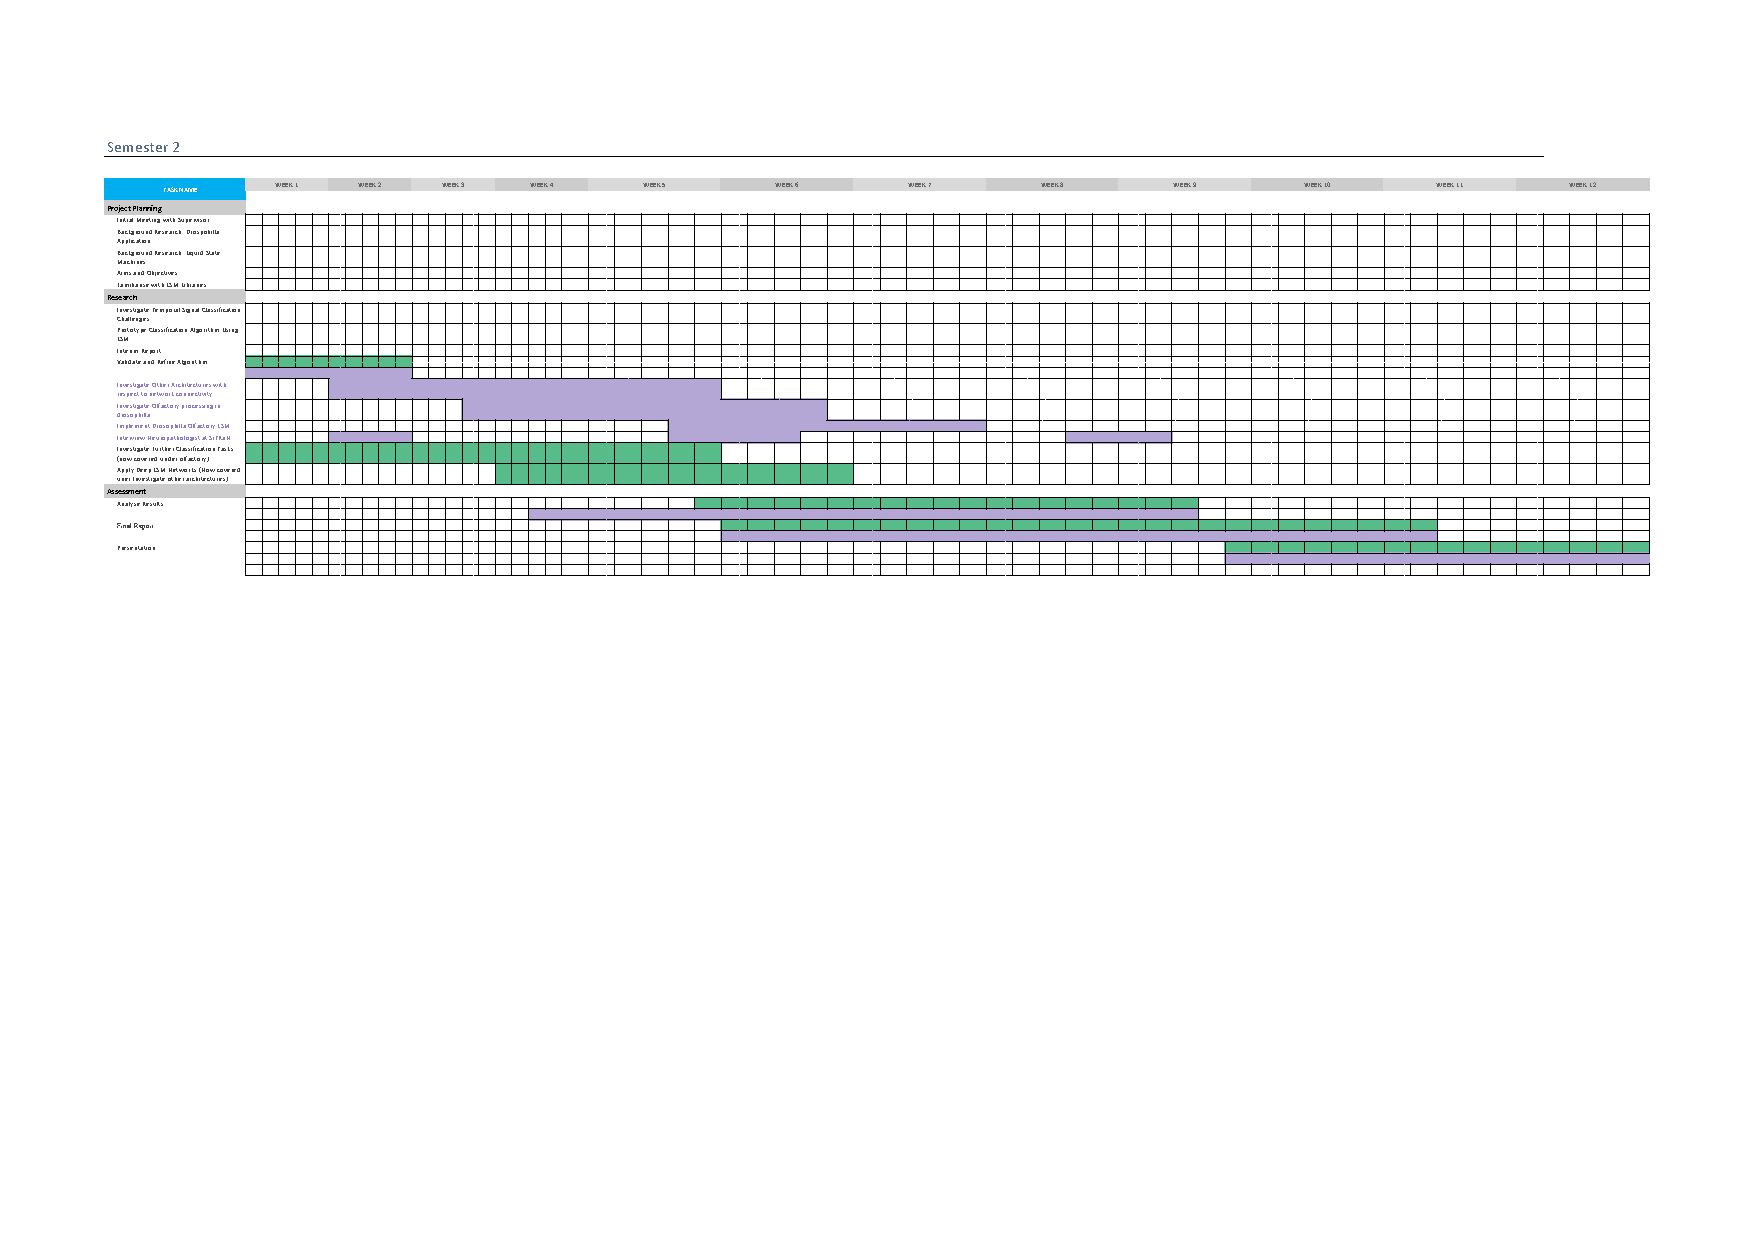
\includepdf[pages=-,angle=90]{chart2.pdf}


\end{document}